\chapter{Theoretical background}
\label{sec:theory}
In this chapter, we give an overview of the theoretical background necessary for Higgs boson searches at the LHC. We start with an overview of the standard model (SM) of particle physics, followed by a description of the phenomenology of proton-proton collisions and Higgs boson production. We conclude with a discussion on the relevance of the search for the associated production of the Higgs boson with top quarks.

\section{The Standard Model}
The fundamental building blocks of the SM are complex quantum fields~$\phi(x)$~that depend on the space-time coordinates~$x$. The interaction of these fields is governed by Quantum Field Theory (QFT). These fields can be classified according to their transformation properties under various symmetry groups, in particular the Lorentz group, and thus associated to particle states. The principle of gauge invariance allows us to use these transformation properties to describe fundamental interactions via particle exchange. Much of particle physics is concerned with the measurement of decay rates and scattering cross sections, which are computed using perturbation series in QFT.

The particle content of the SM is summarised in~\cref{fig:standard_model}, where we see that the fundamental particle states can be grouped into bosons with integer spin and fermions with spin $1/2$. The fermions are divided into quarks that carry colour charge, fractional electric charge and weak isospin, and leptons which are divided into charged leptons and neutrinos and carry no colour charge. In the following, we describe the types of fields in the QFT description of particle physics.

\begin{figure}
\begin{centering}
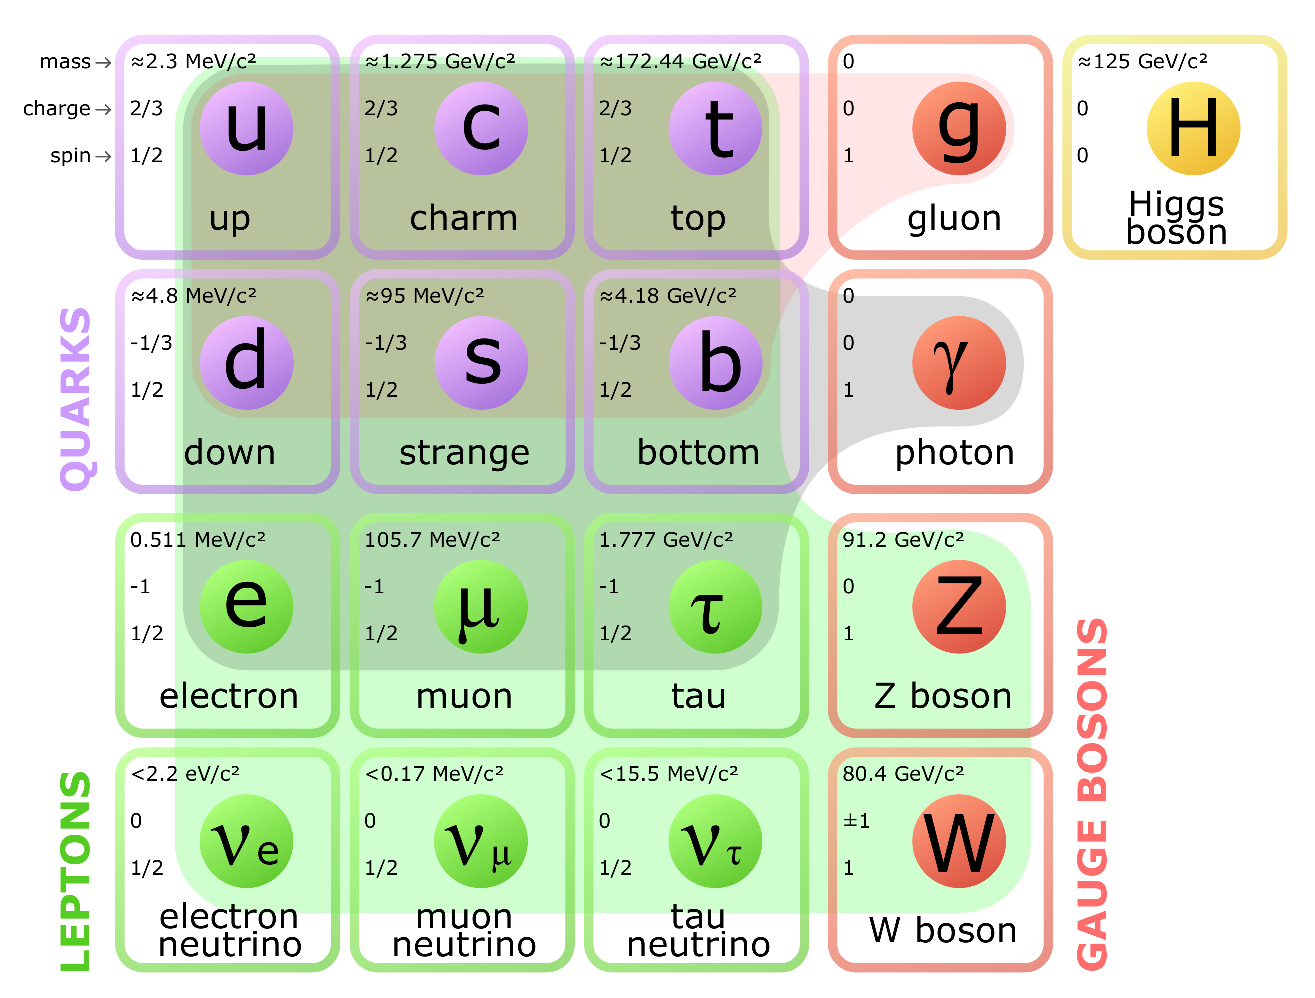
\includegraphics[width=0.8\textwidth]{figures/theory/Standard_Model_of_Elementary_Particles_modified_version.eps}
\caption[The particle content of the Standard Model]{The particle content of the Standard Model. Figure adapted from~\cite{wikipediaSM}.}
\label{fig:standard_model}
\end{centering}
\end{figure}


\subsection{The Lorentz group and particle states}

The Lorentz group consists of coordinate transformations~$x^\mu = \Lambda^{\mu}_{\ \nu} x^\nu$~that preserves the space-time interval~$\mathrm{d}s^2 = \mathrm{d}x^\mu \eta_{\mu\nu} \mathrm{d}x^\nu$ defined through the metric tensor $\eta_{\mu\nu}$. The Lorentz transformation satisfies $\Lambda^{\mu}_{\ \rho} \eta^{\rho\sigma} \Lambda^{\nu}_{\ \sigma} = \eta^{\mu\nu}$, such that~$\mathrm{det}\ \Lambda = +1$~and~$\mathrm{sign}\ \Lambda^0_{\ 0} = +1$. The transformations form a group~$\mathrm{SO}^+(3,1)$, which can be decomposed~$\mathrm{SO}^+(3,1) \simeq \mathrm{SU}(2)_L \times \mathrm{SU}(2)_R$. This allows the angular momenta~$(j_1, j_2)$~of the decomposition to be used to group the fields as scalars~$(j_1=0, j_2=0)$, left and right handed spinors~$(\frac{1}{2}, 0), (0, \frac{1}{2})$ and vectors $(1, 1)$ based on their transformation properties under the Lorentz group. For example, a scalar field~$\phi(x)$~transforms as~$\phi(x) \rightarrow \phi(\Lambda^{-1} x)$, a vector field as~$A^\mu(x) \rightarrow \Lambda^\mu_{\ \nu} A^\nu(\Lambda^{-1}x)$~and a spinor field as~$\phi^\alpha(x) = S[\Lambda]^\alpha_{\ \beta} \phi^\beta(x)$, where~$S[\Lambda]$~is a spinor built from~$4\times4$~Dirac~$\gamma$~matrices in the chiral representation.

These fields can be identified with particle states, which have a definite mass~$m$~and spin~$s$~\cite{wigner1939unitary}. According to the spin-statistics theorem, particles with integer spin (bosons) follow Bose-Einstein statistics, whereas particles with half-integer spin (fermions) follow Fermi-Dirac statistics~\cite{pauli1940connection}. 

\subsection{Relativistic quantum mechanics}
After having identified quantum fields with definite Lorentz transformation properties as the central objects in QFT, the next step is to derive dynamical relations for the free fields in order to describe the propagation of free particles.

The Klein-Gordon wave equation,

\begin{equation}
\label{eq:theory_klein_gordon}
(\partial^\mu \partial_\mu + m^2) \psi = 0
\end{equation}
which can be derived from Einstein's energy-momentum relation~$E^2 = \vec{p}^2 + m^2$~by replacing energy and momentum with operators acting on the wavefunction~$\psi$, is a manifestly Lorentz-invariant relation between energy and momentum for the quantum mechanical wavefunction. However, it admits solutions with negative energy and negative probability densities, which are unphysical.

These negative-probability states led Dirac to search for a relation linear in~$\hat{\mathbf{p}}$~and~$E$, which resulted in the Dirac equation:

\begin{equation}
\label{eq:theory_dirac}
i (\gamma^\mu \partial_\mu - m) \psi = 0
\end{equation}
where~$\gamma^\mu$~are the~$4\times4$~Dirac~$\gamma$-matrices which satisfy the Clifford algebra anti-commutation relation~$\{ \gamma^\mu, \gamma^\nu \} = \gamma^\mu \gamma^\nu + \gamma^\nu \gamma^\mu = 2 g^{\mu\nu} \mathbb{I}$~and~$\psi$~is a four-component spinor. Using~\cref{eq:theory_dirac}, we can describe the dynamics, spin and magnetic moment of free spin-half fermions. The probability densities predicted by Dirac's equation are positive, but it still admits solutions with negative energy. In the Feynman-Stückelberg interpretation, these~$E<0$~solutions can be interpreted as negative-energy particles moving backwards in time or equivalently as anti-particles moving forwards in time. The predictions by Dirac's equation were spectacularly confirmed by the discovery of the positron in 1932~\cite{anderson1933positive}.

Both of these equations of motion can be derived from a Lagrangian using the principle of least action:

\begin{equation}
\label{eq:theory_action}
S = \int \mathrm{d}^4x\ \mathcal{L}_{\mathrm{free}},\quad \delta S = 0,
\end{equation}
where~$\mathcal{L}_{\mathrm{free}}$~is the Lagrangian density for non-interacting fields for the Klein-Gordon or Dirac case respectively and the integral is taken over all possible path variations of the fields. The Dirac action for a single free spinor field can be written as

\begin{equation}
\label{eq:theory_kg_lagrangian}
\mathcal{L}_{\mathrm{Dirac}} = \bar{\psi} i \gamma^\mu \partial_\mu \psi - m \bar{\psi} \psi,\quad \bar{\psi} = \psi^\dagger \gamma^0
\end{equation}
and varied with respect to~$\psi$~to derive the Dirac equation.

\subsection{Interactions via gauge theory}
The concept of interactions mediated by fields is central to QFT. In order to encode the observed particle interactions in the theory, we require the Lagrangian to have additional symmetries. In particular, if we require the laws of physics to be invariant under local transformations~$\psi(x) \rightarrow U(x) \psi(x)$, where the continuous and differentiable transformations~$U(x)$~form Lie groups, then the principle of gauge symmetry allows additional degrees of freedom corresponding to the mediator fields or gauge bosons to be naturally incorporated in the Lagrangian. First, we show how quantum electrodynamics, the relativistic quantum theory of electron-photon interaction and thus electromagnetism, arises from the gauge principle.

\subsection{Quantum Electrodynamics}
For the~$\mathrm{U}(1)$~symmetry, which corresponds to the transformation~$\psi(x) \rightarrow e^{i q\varphi(x)} \psi(x)$, in order for the Lagrangian to be invariant under this symmetry, the derivative in the momentum operator in~\cref{eq:theory_kg_lagrangian} needs to be changed to

\begin{equation}
\partial_{\mu} \rightarrow \mathcal{D}_{\mu} = \partial_{\mu} + i q A_{\mu}(x).
\end{equation}
This ensures that the covariant derivative $\mathcal{D}_{\mu}\psi$ transforms as the field $\psi$ itself under the gauge transformation $U$.
The field~$A_{\mu}$~corresponds to a massless gauge boson with spin 1 that is coupled to the fermion field~$\psi$~via a coupling constant~$q$~in the term~$q \gamma^\mu A_\mu \psi$. The formulation of quantum electrodynamics (QED) as a gauge theory generated by the Abelian group~$\mathrm{U}(1)_{\mathrm{EM}}$~was first done by Tomonaga, Feynman and Schwinger~\cite{PhysRev.73.416, PhysRev.74.1439, PhysRev.76.769}. In QED, the spinor~$\psi$~is associated to the electron, the vector~$A_\mu$~to the photon and~$q$~is the electric charge of the fermion. 

In order to compute observable decay rates or scattering cross sections under an interaction Hamiltonian~$V$, we use Fermi's golden rule, which relates the scattering rate~$\Gamma_{fi}$~to the transition matrix element between the initial and final state derived using perturbation theory:

\begin{equation}
\label{eq:transition_matrix}
\Gamma_{fi} \propto |\mathcal{M}_{fi}|^2 \rho,\quad \mathcal{M}_{fi} = \langle \psi_f | V | \psi_i \rangle
\end{equation}
where $\rho$ is the density of final states which generally depends on the final state energy $E_f$.

The matrix element in~\cref{eq:transition_matrix} is a Lorentz scalar and can be explicitly computed from the Lagrangian using Feynman rules~\cite{Feynman:1948ur}, where we represent each term in the perturbation expansion of~\cref{eq:transition_matrix} as a graphical diagram with the ingoing and outgoing lines. The vertices and the propagators are associated with quantities that are specified by the form of the interaction Lagrangian. The basic QED interaction vertex thus allows us to construct diagrams corresponding to any QED interaction and calculate scattering cross sections for processes such as electron-electron scattering, as depicted in~\cref{fig:theory_qed}.

\begin{figure}
\begin{centering}
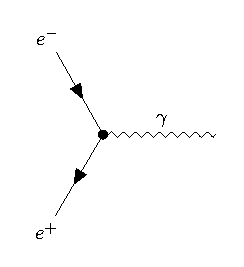
\includegraphics{figures/theory/feyn/qed1.pdf}\\
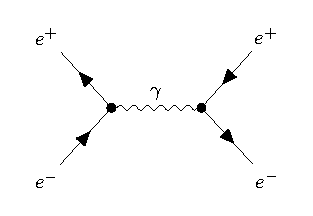
\includegraphics{figures/theory/feyn/qed2.pdf}
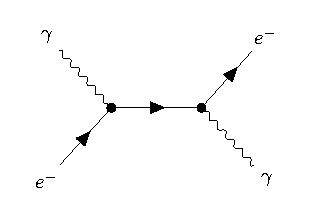
\includegraphics{figures/theory/feyn/qed3.pdf}
\caption{The basic QED vertex (top), a representative leading order diagram for $\mathrm{e}^+ \mathrm{e}^-$ annihilation and subsequent pair production (left) and for Compton scattering (right). Time flows left to right. These figures were created using the \texttt{tikz-feynman} package~\cite{Ellis:2016jkw}.}
\label{fig:theory_qed}
\end{centering}
\end{figure}

It is remarkable that the gauge theory formulation of QED allows us to both recover Maxwell's equations of electromagnetism and predict the anomalous electric dipole moment of the electron, which has been confirmed to be accurate to about one part per billion~\cite{Aoyama:2007mn}. This underscores the predictive power of symmetries in the SM.

\subsection{Quantum Chromodynamics}
\label{sec:theory_qcd}
The interaction of quarks and gluons can be described by the theory of quantum chromodynamics (QCD), which arises from the invariance of the Lagrangian under a local~$\mathrm{SU}(3)_C$~symmetry, where C stands for a colour charge that is~$N_c$-valent, with~$N_c = 3$~in the SM. The spinor field transforms under this group as

\begin{equation}
\psi(x) \rightarrow \psi'(x) = \exp \bigl[ i g_s \alpha^a(x) T^a \bigr] \psi(x)
\end{equation}
where~$T^a$~are the generators of the group represented by the~$3\times3$~Gell-Mann matrices~$\lambda^a$~as~$T^a = \frac{1}{2} \lambda^a$,~$g_s$~is the gauge coupling and~$\alpha^a(x)$~are the local gauge transformations corresponding to the eight generators. The covariant derivative can then be written as


\begin{equation}
\label{eq:theory_qcd_deriv}
\partial_\mu \rightarrow \mathcal{D}_\mu = \partial_\mu + i g_s G^a_\mu T^a
\end{equation}
where~$G^a_\mu$~must transform as~$G^a_\mu \rightarrow G^a_\mu - \partial_\mu \alpha^a - g_s f_{ijk} \alpha^i G^j_\mu$. The last term arises from the non-Abelian nature of QCD, which means that the generators~$T^a$~do not commute, but are instead related through the structure constants:~$[T^a, T^b] = T^a T^b - T^b T^a = 2 i f_{abc} T^c$. The Lagrangian for a single quark field can then be written as

\begin{equation}
\label{eq:theory_quark_lagrangian}
\mathcal{L}_{\mathrm{quark}} = \bar{\Psi} (i \gamma^\mu \partial_\mu - m + g_s \gamma^\mu G^a_\mu T^a) \Psi
\end{equation}
and we can associate~$G^a_\mu$~to the gluons. We note that~$\Psi = (\psi_i)$~has three components corresponding to colour states, each of which is a 4-component Dirac spinor. The QCD quark-gluon interaction vertex is then

\begin{equation}
- g_s \bar{\Psi} \gamma^\mu G^a_\mu T^a \Psi.
\end{equation}

At this stage,~$G^a_\mu$~is simply a field associated with external sources, which can be made dynamical by adding a gauge-invariant term

\begin{equation}
\mathcal{L}_{\mathrm{gauge}} = - \frac{1}{2} \mathrm{Tr}\ [F^{\mu\nu} F_{\mu\nu}] 
\end{equation}
to the QCD Lagrangian, where~$F_{\mu\nu} = \partial_\mu G_\nu - \partial_\nu G_\mu + i g_s [G_\mu, G_\nu]$, with $G_\mu = G_\mu^a T^a$, is the QCD gluon field strength tensor. The non-vanishing structure constants $f_{abc}$ imply that gluons carry colour charge and thus interact with each other, giving rise to a triple-gluon vertex (ggg) proportional to $g_s$ and a 4-gluon vertex (gggg) proportional to $g_s^2$.

The~$\mathrm{SU}(3)_{\mathrm{C}}$~symmetry of QCD thus implies the existence of a conserved trivalent colour charge, which is exchanged between quarks by eight gluons carrying colour-anticolour in QCD vertices. As free quarks have not been experimentally detected, the colour charge is hypothesized to be confined, such that quarks are only observed bound to colourless hadrons - mesons ($\mathrm{q}\bar{\mathrm{q}}$) and baryons (qqq). Furthermore, this means that hadrons have to be colour singlets, which for baryons, composed of three quarks, implies that the colour wavefunction must be totally antisymmetric under the exchange of any two quarks, since the colour  singlet~$\psi_c = \frac{1}{\sqrt{6}} (rgb - rbg + gbr - grb + brg - bgr)$~from the decomposition~$\mathbf{3}\otimes \mathbf{3} \otimes \mathbf{3} = \mathbf{10} \oplus \mathbf{8} \oplus \mathbf{8} \oplus \mathbf{1}$~is totally antisymmetric.

The success of QCD in describing the phenomenology of high-energy interactions of protons relies on a model for building hadrons out of the elementary constituents of QCD - the quarks and gluons.

\subsection{Hadrons}
The known quarks of the SM come in six different flavours, grouped into three generations: up and down (I), charm and strange (II), top and bottom (III). The underlying reason for the SM having exactly three generations is unknown, but an approximate symmetry between flavours allows us to predict allowable hadronic states that can be formed from quarks. Strong interaction is approximately invariant under~$\mathrm{u} \leftrightarrow \mathrm{d}$~exchange, which implies an~$\mathrm{SU}(2)$~flavour symmetry. This group has three generators~$\hat{T}_i$~that can be represented as~$2\times2$~Pauli spin matrices. This means that for a given flavour state~$\psi$, the quantised isospin~$I_3 \leftrightarrow \hat{T}_3$~and the total isospin~$I \leftrightarrow \hat{T}^2$~are conserved in analogy to spin, and can therefore be used to label composite states of quarks as~$\phi(I, I_3)$.

We can construct the flavour wavefunction proton, which contains three valence quarks (uud), by combining three isospin doublets~$\mathbf{2} \otimes \mathbf{2} \otimes \mathbf{2} = \mathbf{4} \oplus \mathbf{2}$, which results in a spin~$I=3/2$~quadruplet and two spin~$I=1/2$~doublets~$\phi_A=\frac{1}{\sqrt{2}}(\mathrm{udu} - \mathrm{duu})$~and~$\phi_S = \frac{1}{\sqrt{6}}(2 \mathrm{uud} - \mathrm{duu} - \mathrm{udu})$, that are (anti)symmetric under the exchange of the first two quarks. The proton wavefunction is then a superposition of the two flavour doublets, multiplied by the corresponding (anti)symmetric wavefunctions for the spin states, such that the flavour-spin wavefunction is completely symmetric under the exchange of any two quarks. This, combined with the completely antisymmetric colour wavefunction described in~\cref{sec:theory_qcd}, guarantees that the proton wavefunction is completely antisymmetric under the exchange of any two quarks.

The~$\mathrm{SU}(2)$~isospin symmetry of flavour allows us to write down the wavefunction of the proton in the ground state and predict the existence and approximate masses of the excited states such as the~$\Delta$-baryons. It is not an exact symmetry, as illustrated by the difference in the proton and neutron masses, which should vanish under precise~$\mathrm{SU}(2)$~isospin symmetry, but nevertheless underscores the role of symmetries in describing hadronic states. Further hadronic states can be described by the $\mathrm{SU}(3)$ model, where the u, d and c quarks are grouped into a triplet

\subsection{Weak interaction}
The weak force is responsible for radioactive~$\beta$-decay and the leptonic decay of mesons. It is the only fundamental interaction known to violate parity~\cite{Wu:1957my}. The weak interaction couples neutrinos to charged leptons and up-type quarks to down-type quarks via the exchange of massive vector bosons, the charged W-boson and the neutral Z-boson. At low energy ($q \ll m_W$) and before the observation of parity violations, the weak force was modelled as a Fermi theory with a matrix element $\mathcal{M} = G_F g_{\mu\nu} [\bar{\psi}_3 \gamma^\mu \psi_1][\bar{\psi}_4 \gamma^\mu \psi_2]$ corresponding to a point interaction of four fermions proportional to the Fermi constant $G_F$. After the observation of parity violation, the weak interaction vertex needed to be modified to include axial vector coupling in addition to vector coupling, such that it is proportional to $g \gamma^\mu(1 - \gamma^5)$. The $\gamma^5$ operator serves to project out the left (right) handed (anti)-particle chiral states, such that only these states interact via weak boson exchange.

The weak interaction can be described in the SM as a~$\mathrm{SU}(2)_L$~gauge symmetry. The left-handed fermions form doublets~$(\nu_L, \mathrm{\ell}_L)$~for leptons and~$(q_L, q'_L)$~for quarks, whereas right-handed fermions $\ell_R$, $q_R$ are singlets under weak isospin. The generators~$T_i$~of~$\mathrm{SU}(2)_L$~are related to the three Pauli matrices~$T_i = \frac{1}{2}\sigma_i$, which can then be associated to two charged vector boson fields that mediate the weak force:~$W^{\pm}_\mu=\frac{1}{\sqrt{2}}(W^1_\mu \mp i W^2_\mu)$. The gauge structure predicts the existence of a massive electrically neutral vector boson $W^3_\mu$, which can be associated to the SM Z boson through electroweak unification, described in the following section.

\subsection{Electroweak unification}

The weak and electromagnetic forces both suggest an electrically neutral boson, so the physically observed states of the photon and the Z-boson must be superpositions of the two, implying a connection between the weak and electromagnetic forces. The mixing between the neutral gauge boson states can be expressed as $A = B \cos{\theta_W} + W^3 \sin{\theta_W}$ and is characterised by the weak mixing angle $\theta_W = \tan^{-1}{g'/g}$ between a new $\mathrm{U}(1)_Y$ gauge field B with a coupling $g'$ and the neutral component of the weak force $W^3$. In the Glashow-Weinberg-Salam theory of electroweak unification~\cite{Glashow:1961tr,PhysRevLett.19.1264,Salam:1968rm}, the Lagrangian is symmetric under the group~$\mathrm{SU}(2)_L \times \mathrm{U}(1)_Y$, whereas the vacuum state is symmetric only under the QED gauge symmetry~$\mathrm{U}(1)_{\mathrm{EM}}$. In the unified theory, it is necessary to introduce a new quantum number~$Y$, the hypercharge, which is equal for both components of the~$\mathrm{SU}(2)_L$~doublets, so that the left-handed doublets would be invariant under both~$\mathrm{SU}(2)_L$~and~$\mathrm{U}(1)_Y$~symmetries. The observed electric charges of the fermions are then related to the weak hypercharge~$Y$~and weak isospin~$I_3$~by~$Q = I_3 + Y/2$.

The theory of electroweak unification was confirmed by the observation of weak neutral currents in the Gargamelle detector~\cite{Hasert:1973ff} and the following discovery of the W and Z-boson by the UA1 and UA2 experiments at the SPS collider~\cite{Arnison:1983mk}, which couples to both left-handed and right-handed fermions. This has allowed the weak mixing angle~$\theta_W$~between the neutral vector boson states to be measured. The principle of local gauge invariance has great predictive power for the overall structure of the observed interactions, but it does not account for the mechanism by which electroweak symmetry breaking (EWSB) is realised nor the mass of the~$\mathrm{W}^\pm$~and Z bosons, which would violate gauge invariance. In order to incorporate these phenomena, we turn to the Higgs mechanism. The decay~$\mathrm{Z} \rightarrow \nu \bar{\nu}$~can be used to determine the number of light neutrino generations by measuring the total width of the Z-boson~$\Gamma_Z$~and the decay widths to visible fermions - the charged leptons~$\mathrm{e}^\pm, \mathrm{\mu}^\pm, \mathrm{\tau}^\pm$~and quarks~\cite{Akrawy:1989pi}.

\subsection{Higgs mechanism}
We can introduce mass terms for the heavy gauge bosons by coupling them to two complex scalar fields arranged in a weak isospin doublet~$\phi = \frac{1}{\sqrt{2}} (\phi^+\ \phi_0)^T$~\cite{Higgs:1964ia,Higgs:1964pj,Englert:1964et,Guralnik:1964eu}. The Lagrangian density for this scalar field is~$\mathcal{L}_{\phi} = (\partial_\mu \phi)^\dagger (\partial^\mu \phi) - V(\phi)$, where the Higgs potential~$V(\phi) = \mu^2 (\phi^\dagger \phi) + \lambda (\phi^\dagger \phi)^2$~has degenerate minima~$\phi^\dagger \phi = v^2 / 2 = -\mu^2/2\lambda$~for~$\mu^2 < 0$. If the physical vacuum state does not have the same symmetries as the Lagrangian, then it is possible to introduce gauge-invariant mass terms for gauge bosons and fermions.

The Higgs field couples to the gauge fields through the kinetic term~$(\partial_{\mu} \phi)^\dagger (\partial^\mu \phi)$, which is made gauge invariant by~$\partial_\mu \rightarrow D_\mu = \partial_\mu + i g T^a W_\mu^a + i g' Y B_\mu / 2$. The vacuum state is then chosen to be~$\langle 0|\phi|0\rangle = \frac{1}{\sqrt{2}} (0\ v)^T$, so the Higgs field can be expanded around the vacuum, resulting in a massive scalar field~$\eta$~and three massless Goldstone fields~$\phi_1, \phi_2, \phi_3$. The Goldstone bosons can be removed from the Lagrangian by fixing the gauge, such that they correspond to the degrees of freedom of longitudinal polarisation states of the Z and~$\mathrm{W}^\pm$~bosons. The masses of the gauge bosons can then be written as~$M_W = \frac{1}{2} g v$~and~$m_Z = \frac{1}{2} g v / \cos{\theta_W}$. The theory of EWSB predicts~$m_W / m_Z = \cos{\theta_W}$, which has been confirmed experimentally~\cite{ALEPH:2005ab}.

The explicit mass terms for fermions in the form of~$m \bar{\psi} \psi$~are not gauge invariant. By arranging the left-handed fermions in $\mathrm{SU}(2)$~doublets~$L$~and the right-handed fermions in singlets~$R$, the mass terms for Dirac fermions can be introduced through spontaneous symmetry breaking through the terms~$y_f \bar{L}\phi R + y_f (\bar{L}\phi R)^\dagger$~for down-type leptons $e^\pm$, $\mu^\pm$, $\tau^\pm$ and quarks $\mathrm{d}$, $\mathrm{s}$~and $\mathrm{b}$. The constant $y_f = \sqrt{2} m_f / v$ is the Yukawa coupling of the fermions, which has to be fixed from the experimental determination of the masses. A conjugate Higgs doublet~$\phi_c = -i\sigma_2 \phi^*$~is used to give the mass terms for the up-type quarks. From this mechanism, the Yukawa coupling of the top quark is found to be compatible with unity, a scale very different from the rest of the quarks.

To summarise, the Higgs mechanism can accommodate the observed masses of heavy gauge bosons and fermions in a unified electroweak theory. It predicts the existence of a massive scalar boson, which can decay to fermions through~$\mathrm{H} \rightarrow \mathrm{f} \bar{\mathrm{f}}$~or bosons through~$\mathrm{H} \rightarrow \mathrm{W}^+ \mathrm{W}^-$ and ~$\mathrm{H} \rightarrow \mathrm{Z} \mathrm{Z}$, and through higher-order processes to $\mathrm{H} \rightarrow \gamma \gamma$.

\subsection{Top quark physics}
The top quark is the most massive particle in the SM, with $m_t = 173.34 \pm \allowbreak 0.27 \mathrm{(stat)} \pm \allowbreak 0.71 \mathrm{(syst)} \GeV$~\cite{ATLAS:2014wva}, such that it is kinematically allowed to decay through weak interaction $\mathrm{t} \rightarrow \mathrm{b} \mathrm{W}^+$. This is the primary decay mode, since $|V_{tb}| \gg |V_{ts}|, |V_{td}|$ from the Cabibbo-Kobayashi-Maskawa mass matrix, which parametrises the strength of the Yukawa interaction between the quarks and the Higgs field~\cite{Cabibbo:1963yz,Kobayashi:1973fv}, and the hadronisation timescale $\Lambda_{QCD}^{-1} \simeq 10^{-23}~\mathrm{s}$ is much larger than the top quark lifetime $\tau \simeq 10^{-25}~\mathrm{s}$. This means that the top quark mass can be measured accurately from a relatively small number of decay products, among which the mesons containing a b~quark have a distinctive experimental signature due to their large lifetime.

The top quark was discovered in 1995 at the CDF experiment at Tevatron~\cite{Abe:1995hr} and is now ubiquitous at the LHC, where it is produced primarily through gluon-gluon fusion in the form of top quark pairs~\cite{Czakon:2013goa}.

%%%%%%%%%%%%%%%%%%%%%%%%%%%%%%%%%%
%%%%%%%%%%%%%%%%%%%%%%%%%%%%%%%%%%
%%%%%%%%%%%%%%%%%%%%%%%%%%%%%%%%%%

\section{The Standard Model at colliders}
\subsection{The parton model}
Through the study of deep inelastic scattering (DIS) experiments, where an electron transfers sufficient four-momentum~$Q^2$~to a proton for it to break up in the process~$\mathrm{e}^- \mathrm{p} \rightarrow \mathrm{e}^- \mathrm{X}$, with $\mathrm{X}$ being a proton remnant, it was possible to establish that the electrons scatter elastically off point-like spin-half constituents of the proton, the partons~\cite{Bjorken:1969ja}. This can be seen as an analogy to the Rutherford experiment, where $\alpha$-particles were scattered off the nucleus of an atom to reveal the point-like structure of the nucleus within. By identifying the partons as the quarks from QCD, electron-proton interactions can thus be described in terms of the more fundamental electron-quark interactions.

Furthermore, by measuring the~$Q^2$-dependence of the QCD coupling constant~$\alpha_s(Q^2) = g_s^2 / 4\pi$~ experimentally and from theoretical considerations of QCD~\cite{PhysRevLett.30.1343,PhysRevLett.30.1346}, it has been possible to establish that at high~$Q^2$, the coupling constant~$\alpha_S(Q^2)$~becomes small ($\alpha_s \simeq 0.1$), such that quarks can be treated as free particles in the asymptotic limit. The~$Q^2$-dependence of~$\alpha_s$~can be seen in~\cref{fig:theory_alphas_running}, confirming the QCD prediction of asymptotic freedom. Only when the coupling~$\alpha_S(Q^2)$~is sufficiently small can perturbative QCD (pQCD) be used to compute cross-sections of the underlying processes. However, it is important to note that the magnitude of the strong coupling constant in the perturbative, high $Q^2$ regime is still significantly larger than the electromagnetic coupling constant, which means that higher-order loop processes are important in QCD.

The other feature of the running of $\alpha_s$ is that at a momentum scale comparable to typical hadron sizes~$\Lambda_{\mathrm{QCD}} = 0.1,\dots0.3$~GeV, the coupling constant becomes very large, implying the breakdown of perturbative QCD at~$Q < \Lambda_{\mathrm{QCD}}$. This means that in processes with low energy scales such as the production or interaction of hadrons, non-perturbative dynamics of QCD become important.

\begin{figure}
\begin{centering}
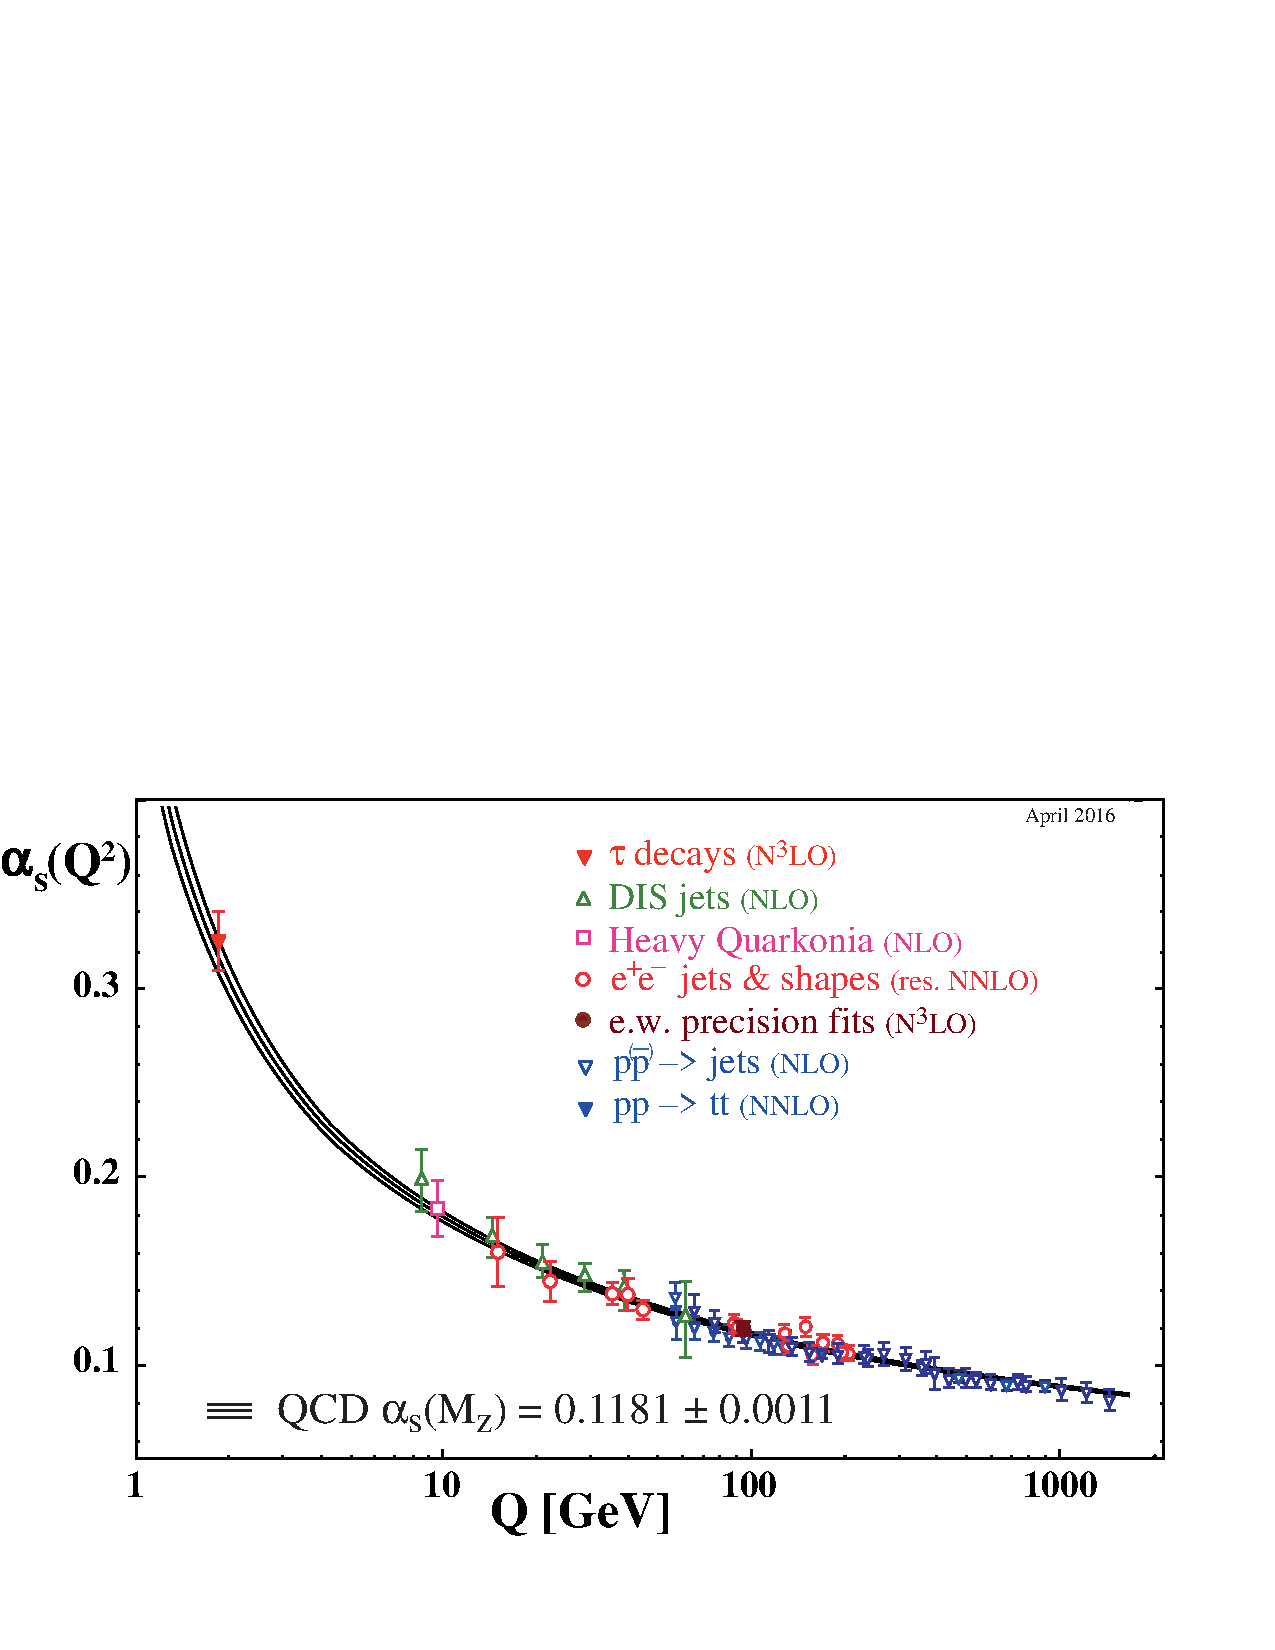
\includegraphics[width=0.6\textwidth]{figures/theory/asq-2015.pdf}
\caption[The measured values of~$\alpha_S(Q^2)$ compared the perturbative QCD prediction]{The measured values of the strong coupling~$\alpha_S(Q^2)$, compared to the prediction from perturbative QCD with five-loop corrections~\cite{Herren:2017osy}. We see that $\alpha_S$ decreases as the momentum scale $Q^2$ increases, reflecting the asymptotically free nature of QCD. Figure from~\cite{Patrignani:2016xqp}.}
\label{fig:theory_alphas_running}
\end{centering}
\end{figure}

In order to model a proton-proton interaction with a hard scattering, such as the Drell-Yan process~$\mathrm{q} \bar{\mathrm{q}} \rightarrow \ell^+ \ell^-$~at high~$Q^2$, we describe the protons in terms of parton distribution functions~(PDFs)~$f_a^{\mathrm{p}}(x)$, which follows from the factorisation theorem in QCD~\cite{collins1989perturbative}. These specify the fraction of proton momentum~$x$~carried by a quasi-free constituent quark or gluon~$a,b$~and factorise the proton-proton interaction to a hard interaction between quarks and gluons, as depicted in~\cref{fig:theory_pdf_factorisation}. This allows us to write the factorised cross-section for the process $\mathrm{p} \mathrm{p} \rightarrow cd$ as

\begin{figure}
\begin{centering}
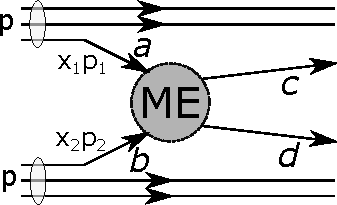
\includegraphics[width=0.4\textwidth]{figures/theory/factorization.pdf}
\caption[An illustration of the factorisation of a proton-proton interaction]{An illustration of the factorisation of a proton-proton interaction to a hard parton-parton interaction.}
\label{fig:theory_pdf_factorisation}
\end{centering}
\end{figure}

\begin{equation}
\label{eq:theory_pdf_factorisation}
\mathrm{d}\sigma(\mathrm{p}\mathrm{p} \rightarrow cd) = \int_0^1 \mathrm{d}x_1 \mathrm{d}x_2 \sum_{a,b} f_a^{\mathrm{p}}(x_1, \mu_F^2) f_b^{\mathrm{p}}(x_2, \mu_F^2)\ \mathrm{d}\hat{\sigma}^{ab \rightarrow cd} (Q^2, \mu_f^2),
\end{equation}
which is evaluated at the factorisation scale~$\mu_F^2$. In a qualitative sense, emissions with a transverse momentum above $\mu_F$ are accounted in the cross-section, otherwise, they are contained in the PDF. As it is not possible to describe the structure of hadrons and the PDFs perturbatively, they have to be determined from experimental data in terms of $x$ and $\mu_F^2$~\cite{Diemoz:1987xu,Ball:2014uwa}. The proton is a dynamical system of bound quarks that interact strongly via virtual gluon exchange, so the protons are found to contain a \textit{sea} of gluons and quarks and anti-quarks from the vacuum fluctuations of~$\mathrm{g} \rightarrow \mathrm{q} \bar{\mathrm{q}}$~in addition to the up and down \textit{valence} quarks expected from flavour symmetry. The PDFs at different scales $\mu_F$ are related through the DGLAP~\cite{Altarelli:1977zs,Dokshitzer:1977sg,Gribov:1972ri}\footnote{Dokshitzer, Gribov, Lipatov, Altarelli and Parisi} evolution equations, which result from QCD corrections and involve splitting kernels that arise from the basic QCD vertices. This allows us to deduce the PDFs at a certain scale from measurements at a different scale, making it possible to use data from various collider experiments in combined PDF fits and for making predictions at the LHC. The PDFs for protons at different factorisation scales are shown in~\cref{fig:proton_pdf}.

\begin{figure}
\begin{centering}
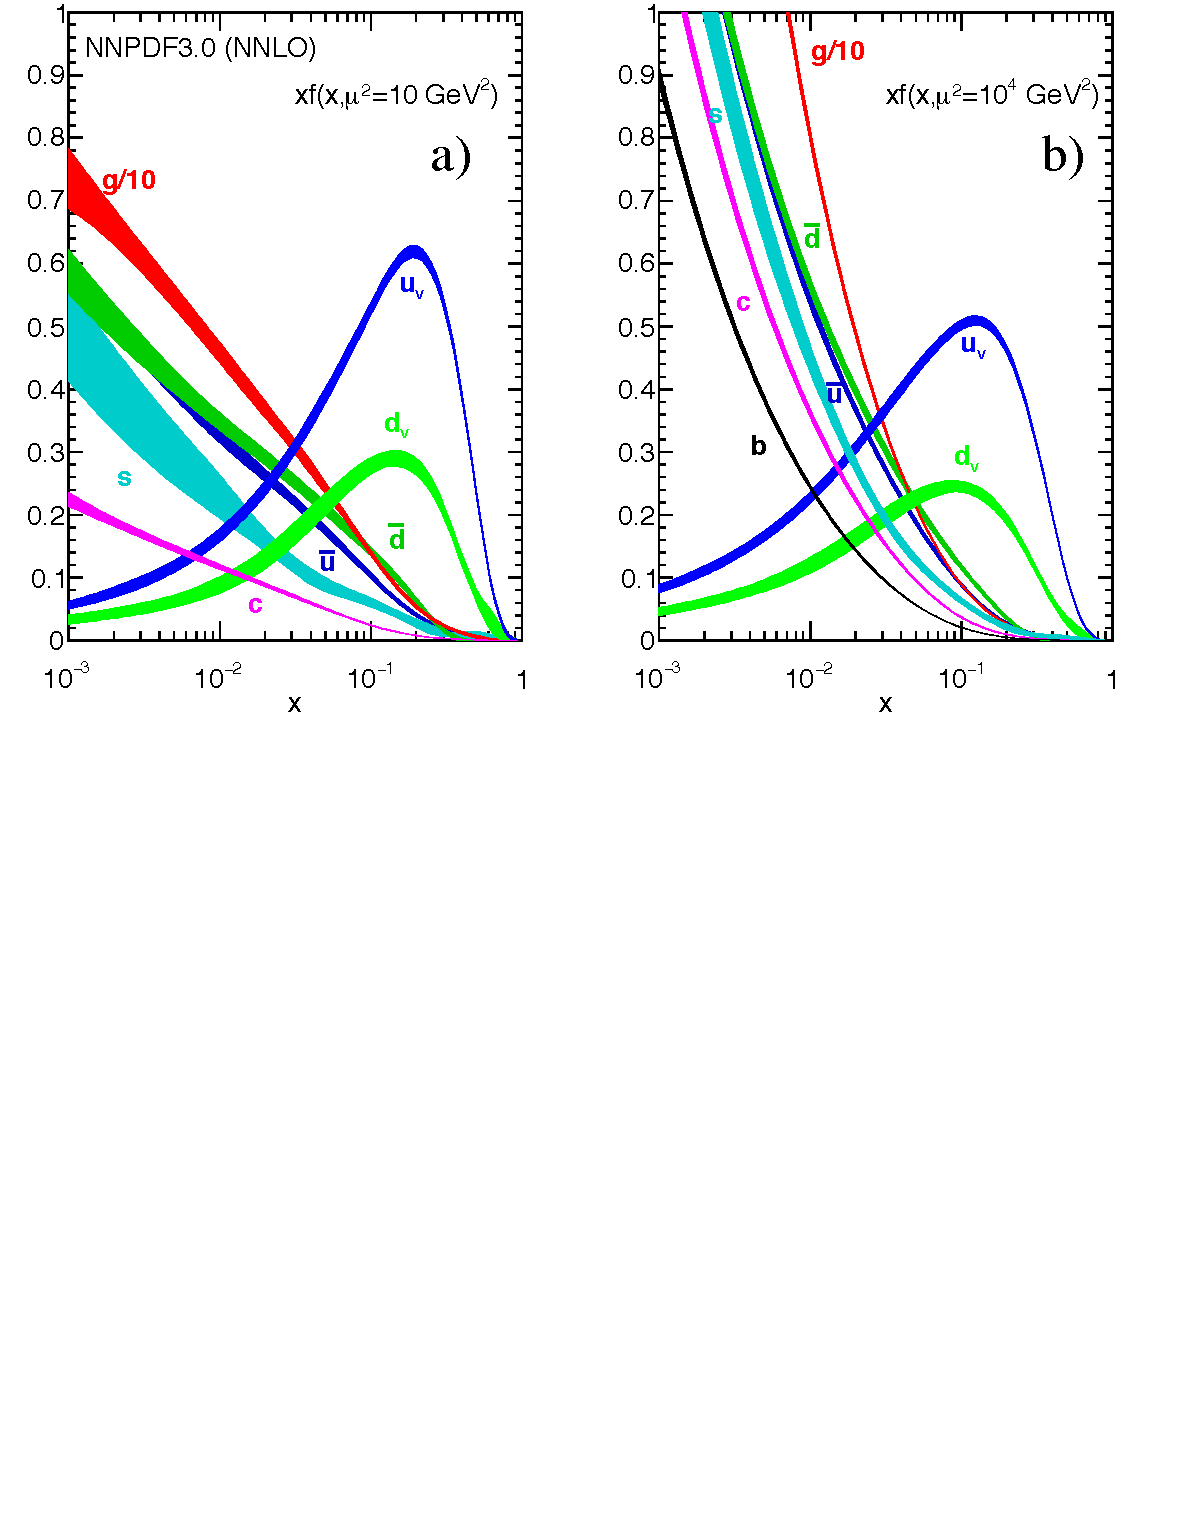
\includegraphics[width=0.8\textwidth]{figures/theory/pdf.pdf}
\caption[The parton distribution functions for protons.]{The parton distribution functions for protons at $\mu_F^2 = 10~\mathrm{GeV}^2$ (left) and $\mu_F^2 = 10^4~\mathrm{GeV}^2$. We see that at higher momenta $\mu_F$ and low $x$, the proton consists almost entirely out of gluons. Figure from~\cite{Patrignani:2016xqp}.}
\label{fig:proton_pdf}
\end{centering}
\end{figure}

\subsection{Jet physics}
In a process where QCD partons (quarks or gluons) are created, we cannot observe them directly, since colour confinement forbids the existence of isolated coloured states. Events with quarks and gluons in the final state can be observed experimentally as collimated jets of hadrons. This feature, which emerges from the short to long distance evolution of QCD, makes it possible to make measurements on macroscopic distance scales and connect them to otherwise inaccessible microscopic quantities such as the parton momenta or quantum numbers~\cite{Sterman:1977wj}.

Jets are formed through the creation of a parton with high virtuality $Q^2$, which undergoes showering until it reaches a soft hadronisation scale, where non-perturbative processes create stable particles, mainly charged pions and protons ($\simeq 60\%$), neutral pions decaying to $\gamma\gamma$ ($\simeq30\%$) and other neutral particles ($\simeq 10\%$). Due to the soft and collinear divergences in the QCD splitting functions, the jets are collimated along the direction of the original parton momentum.

In order to compare QCD predictions to experimental data, jet-related observables must be defined in such a way that they exhibit infrared safety, i.e. stability with respect to the addition of low-$p_T$ particles, and collinear safety, such that the momentum of a single particle can be split up between collinear daughters. Furthermore, they must also be practical to compute for events with very high jet multiplicities that are expected in hadron colliders. This can be done using sequential recombination, where energy clusters with momenta $k_{t,i}$ and corresponding distances $d_{ij} = \mathrm{min}(k_{t,i}^{2p}, k_{t,}^{2p}) \Delta_{ij} / R^2$ are recombined until stable jets can be formed. These jet algorithms are characterised by the jet radius parameter $R$ and the parameter $p$, where $p=-1$ corresponds to the \textit{anti-$k_T$} algorithm~\cite{Cacciari:2008gp}.

\subsection{Monte Carlo event generators}
In order to compute experimental observables such as differential distributions from the underlying theory of the SM, we typically use Monte Carlo (MC) simulators. Although inclusive observables and in some cases differential distributions can be calculated analytically, it is in general not possible to apply experimental cuts, therefore the observable phase space is sampled probabilistically to generate simulated events, which can be compared to the measurement~\cite{Sjostrand:2006za}.

The MC simulators generally have several stages, starting with importance sampling the phase space of the hard scattering process, such that events occur with probability proportional to $|\mathcal{M}|^2$. This is simple at leading order, but in higher orders, the cancellations between real and virtual contributions need to be accounted for and the procedure becomes more complicated~\cite{Frixione:2002ik}. The hard process defines the overall energy flow in the event.

The hard process is followed by the simulation of the parton shower, which evolves down from the hard scale by gluon emission or $\mathrm{g} \rightarrow \mathrm{q} \bar{\mathrm{q}}$ splittings. Showering is generally process-independent, but may depend on the inherent momentum scales in the process. At a scale of around 1 GeV, hadronisation takes over, which is usually treated using phenomenological models~\cite{Andersson:1983ia} for the non-perturbative dynamics. The overall multiplicity of final state particles is defined by the hadronisation models.

Additional radiation from gluon emission and splitting can be generated either at the level of the hard matrix element or in the parton shower in initial (ISR) or final state radiation (FSR). The matching between these two stages is therefore crucially important in accurately predicting the differential distributions, especially for events with high jet multiplicities. Furthermore, all MC implementations contain a number of free parameters, which need to be tuned to experimental data~\cite{Skands:2010ak}.

%%%%%%%%%%%%%%%%%%%%%%%%%%%%%%%%%%
%%%%%%%%%%%%%%%%%%%%%%%%%%%%%%%%%%
%%%%%%%%%%%%%%%%%%%%%%%%%%%%%%%%%%

\section{Higgs phenomenology}
\subsection{Higgs at the LHC}
The discovery of the Higgs boson with $m_H \simeq 125$~GeV in 2012 at the LHC by the CMS~\cite{Chatrchyan:2012xdj} and ATLAS~\cite{Aad:2012tfa} collaborations confirmed the basic mechanism of EWSB and mass generation and completed the particle spectrum of the SM. Following this, a new experimental and theoretical program has opened in experimentally verifying the properties of the Higgs boson. In particular, it should be established whether the Higgs boson couples to SM gauge bosons and fermions as expected by observing these processes directly. In Run 1 of the LHC, the coupling of the Higgs boson to gauge bosons has been established at a relative precision of $\simeq 10\%$, however, to be able to determine the couplings to fermions, Run 2 data of the LHC are necessary~\cite{Khachatryan:2016vau}.

Beyond establishing the existence of the predicted production and decay channels, a crucial test of the Higgs mechanism is determining the coupling strengths of the new scalar field to SM fields and comparing them to the SM predictions. The top quark Yukawa coupling~$y_t$~, which is $\mathcal{O}(10^5)$ times larger than that of the first-generation quarks, determines the evolution of the Higgs self coupling~$\lambda$~under renormalisation and is currently only known indirectly, as will be discussed further in~\cref{sec:top_higgs}. Next, we discuss how the Higgs boson can be produced at the LHC. 

\subsection{Production modes}
The main production modes of the Higgs boson at the LHC, shown in~\cref{fig:higgs_xs}, are through gluon-gluon fusion (ggF), with a cross-section at $\sqrt{s} = 13~\mathrm{TeV}$ of~$\sigma_{\mathrm{ggF}} = 48.6\pm 5\%$~pb, weak or vector boson fusion (VBF) with a cross-section $\sigma_{\mathrm{VBF}} = 3.78\pm2\%$~pb, associated production with vector bosons (VH) with~$\sigma_{\mathrm{WH}} = 1.37\pm2\%$~pb,~$\sigma_{\mathrm{ZH}} = 0.88\pm5\%$~pb and through the associated production with top quark pairs (\ttH) with $\sigma_{\ttH} = 0.50^{+9\%}_{-13\%}$~pb or with a single top quark~(tH)~\cite{Patrignani:2016xqp}. We note that the difference between the cross sections for the ggF and~\ttH~production modes is roughly two orders of magnitude.

\begin{figure}
\begin{centering}
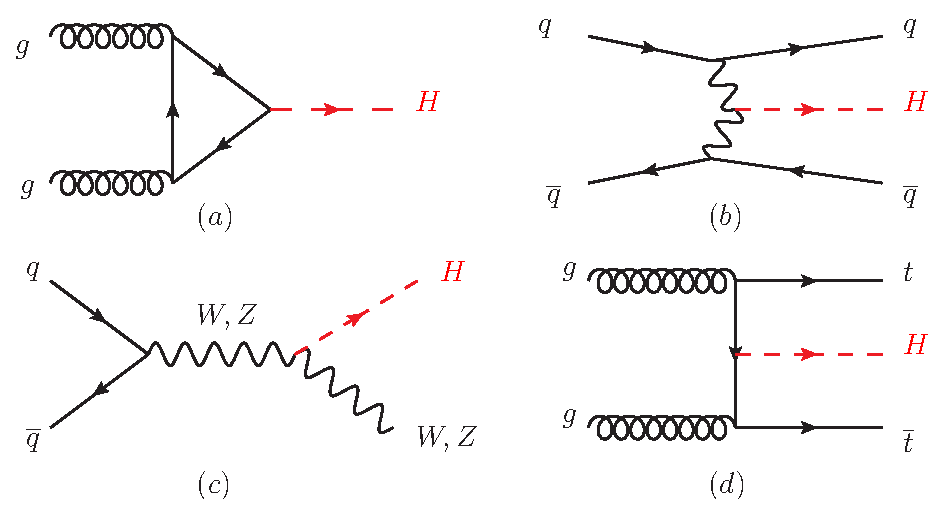
\includegraphics[width=0.8\textwidth]{figures/theory/PDG.eps}
\caption[Tree-level Feynman diagrams for Higgs production]{The generic tree-level Feynman diagrams for Higgs boson production: the gluon fusion process (ggF) (a), vector boson fusion (b), associated production with vector bosons (VH) (c) and associated production with top quarks (\ttH) (d). Figure from the PDG~\cite{Patrignani:2016xqp}.}
\label{fig:higgs_production}
\end{centering}
\end{figure}

\begin{figure}
\begin{centering}
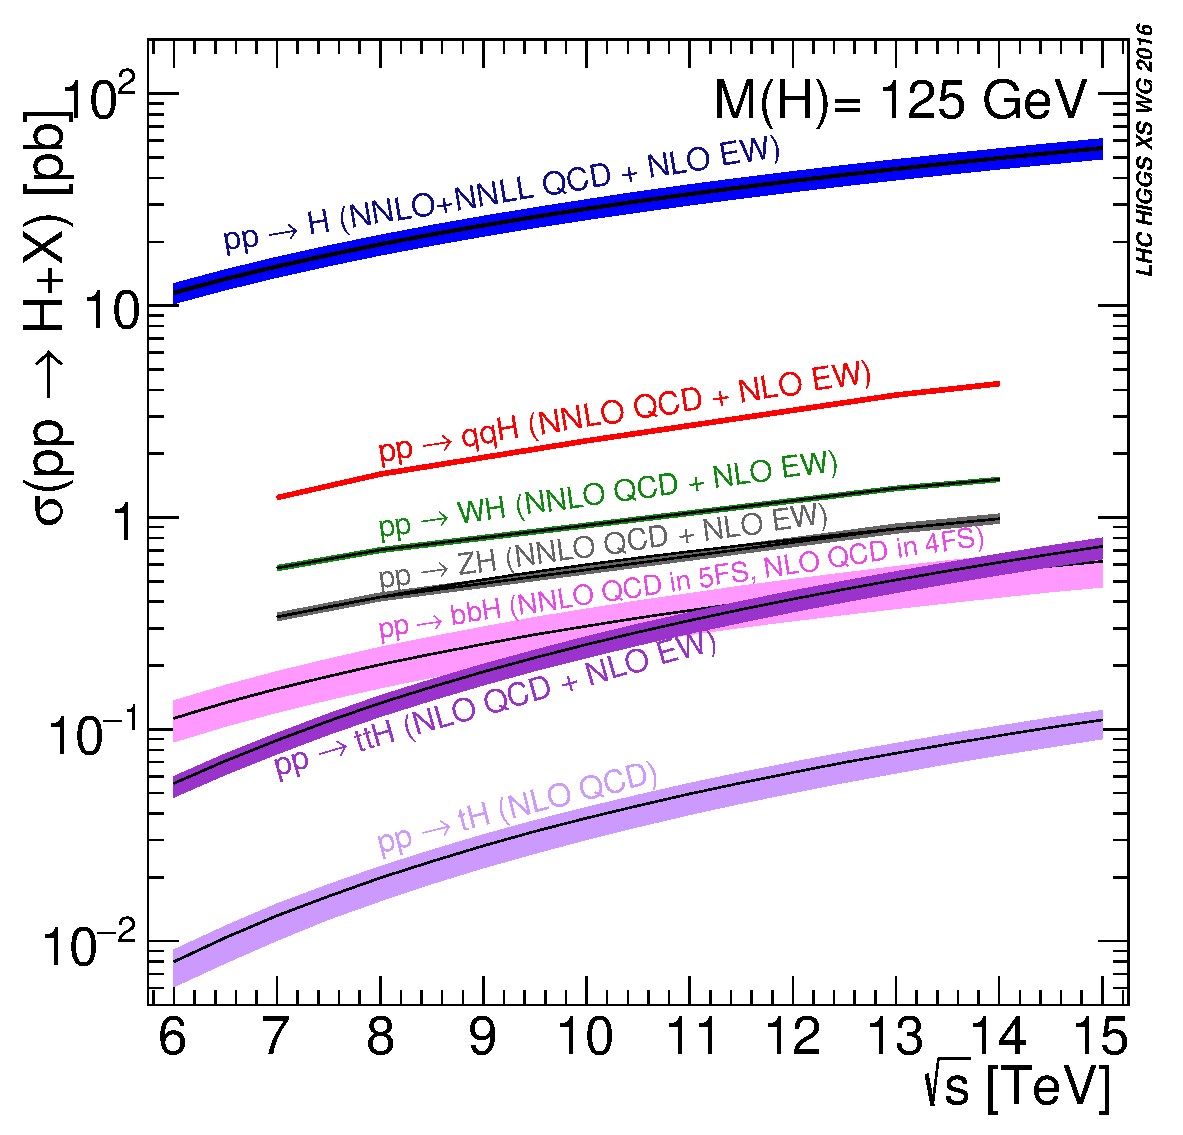
\includegraphics[width=0.5\textwidth]{figures/theory/Higgs_XS_7-14TeV-2016.eps}
\caption[The production cross-section of the Higgs boson]{The production cross section of the SM Higgs boson with $m_H = 125$~GeV as a function of~$\sqrt{s}$ along with theoretical uncertainties. Figure from the PDG~\cite{Patrignani:2016xqp}.}
\label{fig:higgs_xs}
\end{centering}
\end{figure}

The ggF production proceeds predominantly via the top quark loop and is known to N3LO~\cite{Anastasiou:2016cez}. This was the main production mode for the initial observation with the~$\mathrm{H} \rightarrow \gamma \gamma$,~$\mathrm{H} \rightarrow \mathrm{W}^+\mathrm{W}^- \rightarrow \mathrm{e} \mathrm{\nu} \mathrm{\mu} \mathrm{\nu}$~and~$\mathrm{H} \rightarrow \mathrm{Z}\mathrm{Z} \rightarrow 4\ell$ signatures, which are important for the measurement of the production cross-section,~$J^P$~and mass of the Higgs boson. It also serves as an indirect constraint on the top-Higgs Yukawa coupling, due to the presence of the top quark loop in ggF. For the direct decay of the Higgs boson to fermions, which has a higher branching ratio than~$\mathrm{H} \rightarrow \mathrm{\gamma \gamma}$, additional production modes with a lower cross-section can be used. The VBF mode, where two (anti)quarks scatter by exchanging a weak boson in~$\mathrm{qq} \rightarrow \mathrm{qqH}$~is important both for discovery and determination of the couplings, as it can be distinguished from QCD background through the presence of two jets in the opposite forward regions of the detector originating from the scattered quarks. The VH mode allows the use of leptonic decays of the W/Z bosons to reduce the multijet background, such that this mode has recently been used to establish the~\Hbb~decay~\cite{Aaboud:2017xsd}. While inclusive Higgs cross section measurements in the ggF channel are indirectly sensitive to the top quark Yukawa coupling~$y_t$, the~\ttH~and tH channels can be used to probe~$y_t$~directly, such that they provide an important independent verification of the mass generation mechanism for the top quark.

\subsection{Decay channels}
The Higgs boson decays to SM particles with decay widths~$\Gamma$~that are proportional to the mass of the daughter particles. For~$m_H \simeq 125$~GeV, the dominant decay channels are the decay to bottom quarks~\Hbb~with a branching ratio~$\mathrm{BR} = \Gamma/\Gamma_{H} = 0.584 \pm 0.019$, the decay to an on-shell and an off-shell W-boson~$\mathrm{H}\rightarrow \mathrm{W} \mathrm{W}^*$~($\mathrm{BR} = 0.214\pm 0.009 $), the decay to Z bosons $\mathrm{H} \rightarrow \mathrm{Z} \mathrm{Z}$~($\mathrm{BR} = 0.026 \pm 0.001$) and the decay to tau leptons~$\mathrm{H} \rightarrow \mathrm{\tau}^+ \mathrm{\tau}^-$~($\mathrm{BR} = 0.063 \pm 0.004$)~\cite{Patrignani:2016xqp}. Through loop-induced processes, which are enhanced by the large top quark mass, the Higgs boson can also decay to massless particles in the channels~$\mathrm{H} \rightarrow \mathrm{g} \mathrm{g}, \mathrm{\gamma}\mathrm{\gamma}$ with non-negligible branching fractions. The branching ratios for a SM Higgs boson as a function of~$m_H$~can be seen in~\cref{fig:higgs_br}.

\begin{figure}
\begin{centering}
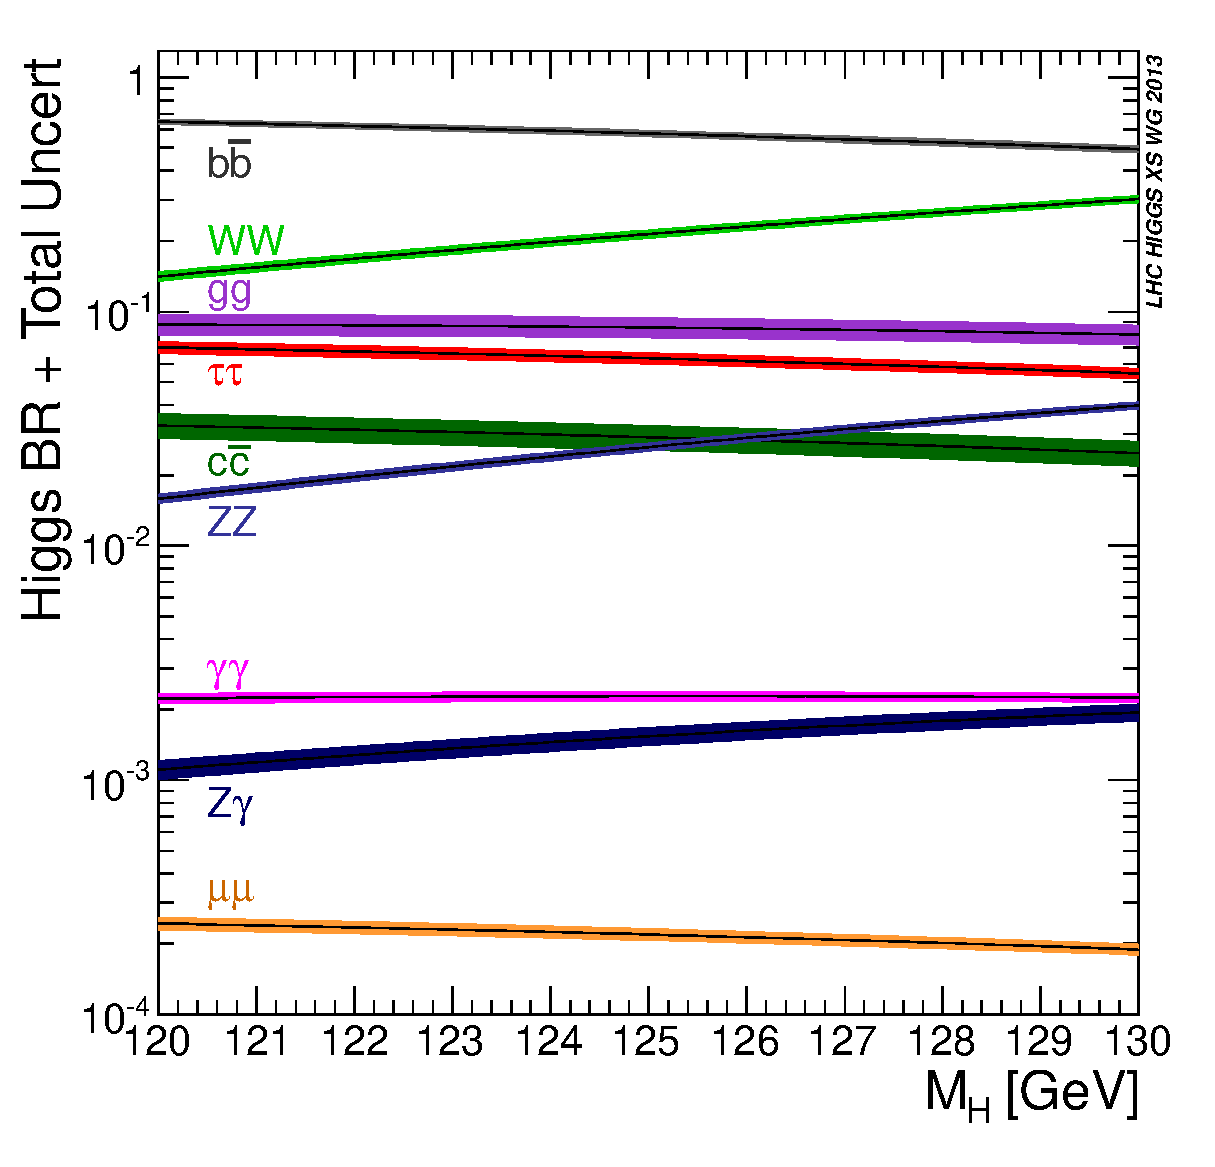
\includegraphics[width=0.5\textwidth]{figures/theory/higgs_br.eps}
\caption[The branching ratios of the Higgs boson]{The branching ratios of the SM Higgs boson around~$m_H = 125$~GeV along with the theoretical uncertainties. Figure from the PDG~\cite{Patrignani:2016xqp}.}
\label{fig:higgs_br}
\end{centering}
\end{figure}

\subsection{Experimental characterisation}
Accurate predictions for the Higgs boson production cross sections and branching ratios for decays allow the interpretation of experimental data and measuring the properties of the Higgs boson in various channels. The mass~$m_H$~has been measured most accurately in the~$\mathrm{H}\rightarrow\mathrm{\gamma}\mathrm{\gamma}$~and~$\mathrm{H} \rightarrow \mathrm{Z}\mathrm{Z} \rightarrow 4\ell$~channels, with a combined value of~$m_H = 125.09 \pm 0.21~(\mathrm{stat}.) \pm 0.11~(\mathrm{syst})$~GeV, dominated by statistical uncertainties, with the photon momentum scale uncertainties being the most significant systematic uncertainty~\cite{Aad:2015zhl}. This has been confirmed in a recent measurement of the Higgs boson properties in the $\mathrm{H} \rightarrow \mathrm{Z}\mathrm{Z} \rightarrow 4\mathrm{\ell}$ channel, where the Higgs boson mass has been determined to be $m_H = 125.26 \pm 0.2~\mathrm{(stat.)} \pm 0.08~\mathrm{(syst.)}$, with the systematic uncertainties dominated by the lepton momentum scale~\cite{Sirunyan:2017exp}. The spin and parity~$J^P$~of the Higgs boson are probed independently of the mass and total cross section and are found to be compatible with the SM~$0^+$ hypothesis, excluding the pseudo-scalar hypothesis at a~$98-99\%$ confidence level~\cite{Khachatryan:2014kca,Aad:2013xqa}. The width of the Higgs boson cannot be measured directly at the LHC, since the mass resolution in the diphoton and~$4\ell$~channels is $1-2$~GeV, three orders of magnitude larger than the expected SM line width $\Gamma_H = 4.2$~MeV~\cite{Patrignani:2016xqp}. However, it can be constrained by comparing the on-shell and off-shell~$\mathrm{H} \rightarrow \mathrm{VV}$~cross sections, thus setting upper limits on~$\Gamma_H$~that are around 5-6 times the SM value~\cite{Khachatryan:2014iha}.

It is important to experimentally confirm that the coupling strengths of the Higgs boson to SM particles correspond to those predicted by the SM. Any deviation from the values predicted by the SM Higgs mechanism could thus signal physics beyond the SM (BSM). The simplest way to experimentally characterise discrepancies in the couplings is the so-called~$\kappa$-framework~\cite{Heinemeyer:2013tqa}, where the couplings to SM particles are rescaled by factors~$\kappa_i$~for~$i \in \{\mathrm{Z}, \mathrm{W}, \mathrm{f}, \mathrm{g}, \mathrm{\gamma}, \mathrm{Z\gamma}\}$~which can be determined from signal strength~($\mu = \sigma / \sigma_{\mathrm{SM}}$)~measurements, without modifying the SM structure of the theory. In this formalism, the~\ttH~signal strength modifier is given by~$\mu_{\ttH} = \kappa_{\mathrm{t}}^2$. The CMS and ATLAS collaborations have extracted these signal modifier values from Run 1 data in a combined fit, with the results shown in~\cref{fig:higgs_kappa}. The couplings, while compatible with the SM, have significant uncertainties, in particular for the Higgs-top quark coupling~$\kappa_t$, thus paving the way for Run 2 measurements with improved sensitivity.

\begin{figure}
\begin{centering}
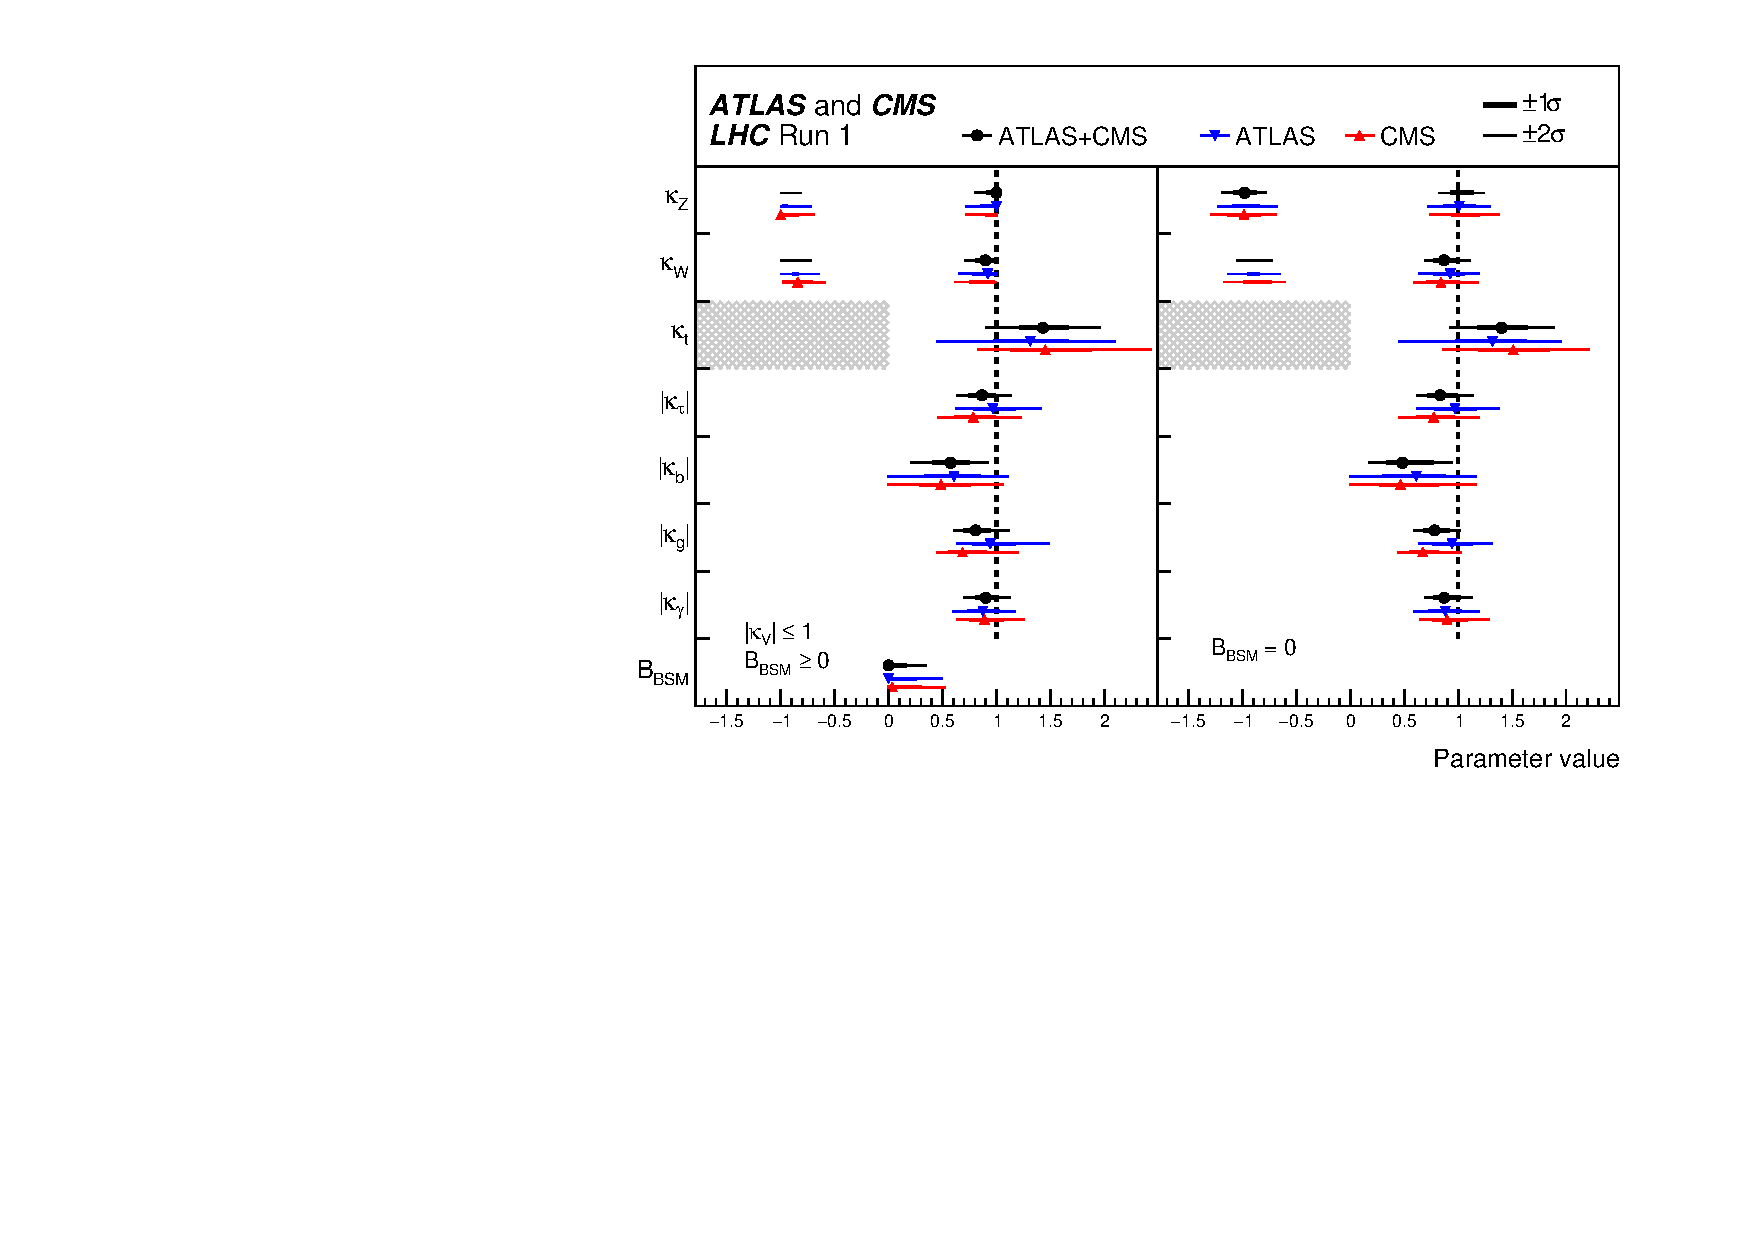
\includegraphics[width=0.8\textwidth]{figures/theory/CMS-HIG-15-002_Figure_015.pdf}
\caption[The Higgs signal strength modifiers as measured by CMS and ATLAS]{The combined signal strength modified factors~$\kappa$~from the CMS and ATLAS collaborations with Run 1 data. Figure from~\cite{Khachatryan:2016vau}.}
\label{fig:higgs_kappa}
\end{centering}
\end{figure}

While the~$\kappa$-framework is relatively simple to apply for small deviations in signal strength, the clear shortcoming of this approach is that any BSM physics would necessarily change the structure of the theory, rendering the results potentially invalid. In particular, the above approach assumes that the loop contributions in ggF and $\mathrm{H} \rightarrow \mathrm{\gamma} \mathrm{\gamma}$ are not modified by new physics. However, contributions with a different Lorentz structure from the SM cannot be captured in the~$\kappa$~framework. Therefore, it has been suggested to use either Higgs pseudo-observables~\cite{Gonzalez-Alonso:2014eva} or effective field theories (EFT) to further parametrise any possible deviations from the SM~\cite{Buchmuller:1985jz,Grzadkowski:2010es}.

\subsection{Top-Higgs coupling}
\label{sec:top_higgs}
In the SM, the coupling between the top quark and the Higgs boson is predicted to be~$y_t = \sqrt{2} m_t / v$, which can be verified by measuring the cross sections of top quark pair associated Higgs production. This implies that the direct determination of the top-Higgs coupling in~\ttH~is a test of the EWSB model at a natural scale where~$y \simeq 1$. 

\subsubsection{Vacuum stability}
The top-Higgs coupling plays an important role in vacuum stability, since it controls the evolution of the self-coupling~$\lambda$~of the Higgs potential through renormalisation evolution $\frac{\mathrm{d}\lambda}{\mathrm{d}\ln{\mu}}$, where it gives a quartic negative contribution. In particular, if~$y_t$~is sufficiently large but well within the bounds set by experimental uncertainties, the self-coupling~$\lambda$~becomes negative at a renormalisation scale~$\mu$~below the Planck scale~$M_{\mathrm{Pl}} = \sqrt{\bar{h}c / G} \simeq 10^{19}~\mathrm{GeV}$, where gravitation becomes important. This means that the Higgs potential develops an additional minimum, which would possibly make the SM vacuum state unstable or metastable, depending on the exact values of~$m_H$~and~$m_t$~\cite{Degrassi:2012ry}. Given that we have not observed a transition between the vacuum states, this would imply the existence of new physics that would prevent this. Since the scale where the scalar self coupling becomes negative depends strongly on~$y_t$, an accurate determination of~$y_t$~can help to pinpoint the scale of new physics in the absence of clear BSM signals~\cite{Bezrukov:2014ina} and establish whether the vacuum is stable on cosmological timescales.

\subsubsection{Anomalous couplings}
Furthermore, the top-Higgs coupling, which is purely scalar in the SM, can be extended quite generally to contain scalar and pseudoscalar interactions, making it possible to use results from~\ttH~for setting direct constraints on anomalous top-Higgs couplings~\cite{Kobakhidze:2016mfx}. Such anomalous couplings can arise from a two-Higgs doublet model~\cite{Lee:1973iz,Branco:2011iw} that appears in several BSM scenarios, such as supersymmetry~\cite{Haber:1984rc}, axions~\cite{Kim:1986ax} or from models with a composite Higgs~\cite{Liu:2017dsz}. Measurements of the \ttH~cross-section can help to constrain such anomalous couplings.

\subsection{Current results on~\ttH}
Both the CMS and ATLAS collaborations have searched for~\ttH~in Run 1 and Run 2 of the LHC by measuring $\mu = \sigma_{\ttH} / \sigma_{\mathrm{SM}}$ in a~\ttH-enriched region using different Higgs decay channels, with the~$\mathrm{H} \rightarrow \mathrm{WW^*},\mathrm{ZZ^*} \rightarrow \mathrm{multilepton}$, \Hbb~and~\Htautau~decay channels providing the highest sensitivity in Run 2, followed by~\ttH-tagged~\Hgg~decay in the diphoton analysis. The results are summarised in~\cref{tab:tth_results}. The analyses are systematically dominated and quite involved in terms of statistical methods. A recent combination by ATLAS while this work was in preparation has been able to measure a cross-section of $\sigma_{\ttH} = 590^{+160}_{-150}~\mathrm{fb}$, compared to the SM value of~$\sigma_{\ttH}^{\mathrm{SM}} = 507^{+35}_{-50}~\mathrm{fb}$, with the equivalent measurement from CMS in the \Hbb~channel being a major part of this thesis.

\begin{table}[h!]
\def\arraystretch{1.5}
\begin{center}
\begin{tabular}{c|cc}
\hline
decay channel & CMS & ATLAS \\
\hline
\multirow{3}{*}{\Hbb} & $\mu = -0.19 \pm 0.45~\mathrm{(stat)} \pm 0.68~\mathrm{(syst)}$ & $\mu = 0.84 \pm 0.29~\mathrm{(stat)} \pm 0.57~\mathrm{(syst)}$ \\
 & $\mu < 1.5~(1.7)~\mathrm{obs~(exp)}$ @ 95\%~CL & $\mu < 2.0~(1.2)~\mathrm{obs~(exp)}$ @ 95\%~CL\\
 & $12.9~\mathrm{fb}^{-1}$~\cite{CMS:2016zbb} & $36.1~\mathrm{fb}^{-1}$~\cite{ATLAS:2017nkr} \\
\hline
\multirow{3}{*}{multi-lepton} & $\mu = 1.5 \pm 0.5$ & $\mu = 1.6^{+0.5}_{-0.4}$ \\
 & $\mu < 2.0~(2.2)$ @ 95\%~CL & $4.1\sigma$~obs ($2.8\sigma$ exp.)\\
 & $35.9~\mathrm{fb}^{-1}$ ($\mathrm{WW^*}, \mathrm{ZZ^*}, \mathrm{\tau_\ell\tau_\ell}$)~\cite{CMS:2017vru} &  35.9~$\mathrm{fb}^{-1}$~\cite{ATLAS:2017lpi}\\
\hline
\multirow{3}{*}{\Htautau} & $\mu = 0.72^{+0.62}_{-0.53}$ & \\
 & $\mu < 1.3~(1.4)$ @ 95\%~CL & included in multi-lepton\\
 & $35.9~\mathrm{fb}^{-1}$ ($\tau_h \tau_l$)~\cite{CMS:2017lgc} &  \\
\hline
\multirow{3}{*}{\Hgg} & $\mu = 2.2^{+0.9}_{-0.8}$ & $\mu = 0.5 \pm 0.6$ \\
 & $3.3\sigma$~obs ($1.5\sigma$ exp.) & $\mu < 1.7~(2.3)$ @ 95\%~CL \\
 &  $35.9~\mathrm{fb}^{-1}$, \ttH~tag~\cite{CMS:2017rli} & $36.1~\mathrm{fb}^{-1}$, \ttH~tag~\cite{ATLAS:2017myr}  \\
\hline
\hline
\end{tabular}
\caption[Current results on~\ttH]{Current results on~\ttH~production from Run 2 of the LHC.}
\label{tab:tth_results}
\end{center}
\end{table}

\section{Summary}
The discovery of the Higgs boson in 2012 has opened up a new field of research in experimentally probing the properties of this fundamental scalar field. Measurements of the Higgs boson are entering the precision era with an increasing attention on rare production and decay modes, which allow the nature of the EWSB mechanism to be verified experimentally. In Run 2 of the LHC, several rare production modes have allowed to confirm the coupling of the Higgs boson to quarks and leptons. Many BSM theories predict changes to the EWSB sector, with the determination of the top quark Yukawa coupling being an important test of the mechanism of mass generation. The LHC experiments are already probing this coupling, but work remains to be done both on the experimental side in reducing measurement uncertainties and on the side of theoretical predictions. The current dataset collected by the CMS and ATLAS experiments is approximately 1\% of the total foreseen over the lifetime of the LHC project, therefore considerable progress can be made in precision measurements of the Higgs boson and thus the SM.